
\chapter{引言}

\section{研究背景}
% \begin{itemize}
%   \item 量子计算的兴起与发展:简要介绍量子计算的历史和发展趋势。
%   \item 量子模型检测的重要性:介绍量子模型检测在量子计算领域中的重要性。(todo: 重要性)
%   \item TDD技术的引入:描述Tensor Decision Diagrams(TDD)技术的引入背景及其在量子计算中的潜在应用。
% \end{itemize}
% //TODO:add some
模型检测(Model Checking)是一种自动化形式方法,用于验证有限状态系统的性质。模型检测最初由 E. M. Clarke 和 E. A. Emerson 提出\citep{Emerson_1980,Clarke,Clarke_1986},如今已广泛应用于软件和硬件设计。例如,在嵌入式系统中,可以使用 UML 活动图来验证硬件是否符合规范\citep{Grobelna_2015}。

模型检测将待检测的系统建模为一个跃迁系统(transition system),在时序逻辑(temporal logic)中指定待验证的属性。给定模型\(M\) 和属性\(\varphi\),模型检测将验证是否\(M\)满足\(\varphi\)。在不同的模型检测方法中,高级符号模型检查(Advanced Symbolic Model Checking)\citep{Grobelna_2015}使用简化的有序二叉决策图(Reduced Ordered Binary Decision Diagrams,ROBDDs 或 BDDs)\citep{Bryant_1986}来表示状态集合和转移关系。通过迭代调用图像计算算法来计算所有可达状态,判断一个模型是否满足时间属性,直到达到不动点为止。

最近,随着量子计算的发展,关于量子线路的验证技术也在不断发展\citep{viamontes2007checking,burgholzer2020advanced}。其中,利用模型检测方法对线路进行自动化验证也有了一些应用。由于量子线路运算空间随着量子比特的线性增加而指数级膨胀,传统的计算方法并不能很好应对。因此本次研究希望应用基于张量网络(tensor network)的张量决策图(tensor decision diagrams)进行量子模型检测。下面简单介绍一下本次研究相关的量子计算和量子模型检测。
\subsection{量子计算简介}
% //TODO:add more intro
量子计算机(quantum computer)是一种利用量子比特特性进行计算的一种设备。在量子计算中,量子比特的特殊性质允许其同时处于多种状态,这与经典比特的二进制状态不同。量子计算机的状态空间可以用希尔伯特空间(Hilbert space)\(\mathcal{H}\)表示\citep{nielsen2010quantum},即可以进行内积运算(inner product)的复向量空间。比特状态可以用\(\mathcal{H}\)的向量表示,量子门由\(\mathcal{H}\)上的酉算子(unitary operator)表示。

量子线路(quantum circuit)是一种描述量子计算的模型。在量子线路中,通过量子比特的初始化、应用量子门、测量以及其他可能的操作的序列来构建和执行量子计算任务。量子线路通常从左向右阅读,每个量子门的作用是将输入的量子比特状态转变为输出状态,该过程可以认为是量子门的酉矩阵与输入的量子状态的乘积。
\begin{figure}[!htbp]
    \centering
    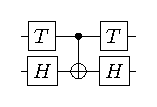
\includegraphics[width=.6\textwidth]{Img/example_cir.pdf}
    \caption{一个量子线路的例子}
    \label{fig:example_cir}
\end{figure}

图\ref{fig:example_cir} 所示的量子线路展示了一个具体的量子线路示例。其中有单比特门\(H=\frac{1}{\sqrt2}\left[\begin{matrix}1&1\\1&-1\\\end{matrix}\right],T=\left[\begin{matrix}1&0\\0&e^{-i\pi/4}\\\end{matrix}\right]\),以及双比特门\(CX=\left[\begin{matrix}\begin{matrix}1&0\\0&1\\\end{matrix}&\begin{matrix}0&0\\0&0\\\end{matrix}\\\begin{matrix}0&0\\0&0\\\end{matrix}&\begin{matrix}0&1\\1&0\\\end{matrix}\\\end{matrix}\right]\)。假设该量子线路的初始状态为\(\left|\psi\right\rangle=\left|\psi_1\right\rangle\left|\psi_2\right\rangle\),则输出状态为\(T\otimes H\cdot CX\cdot T\otimes H\cdot\left|\psi\right\rangle\)。

在量子计算机上可以执行各种算法和计算任务,如量子搜索\citep{Grover_1996}、量子因子分解\citep{shor}和量子模拟\citep{Feynman}等。量子计算的潜力在于其能够在某些特定问题上比经典计算机更高效地进行计算,尤其在处理大规模数据和解决复杂问题方面具有潜在优势。需要对这部分深入了解的读者,可以自行阅读\citep{nielsen2010quantum}。

\subsection{量子模型检测简介}
目前量子的模型检测,主要使用Birkhoff-von Neumann Quantum Logic来描述量子系统的性质\citep{birkhoff1987logic}。Birkhoff-von Neumann量子逻辑是一种非经典逻辑,用于描述量子力学中事件的逻辑结构。它由 Birkhoff 和 von Neumann 在 1936 年首次提出。在量子逻辑中,命题的集合不再形成布尔代数,而是形成一个投影算子的正交完备格,这与传统的逻辑系统不同。

在 Birkhoff-von Neumann 量子逻辑中,量子系统的状态可以由希尔伯特空间(Hilbert space)来描述,每个量子命题对应希尔伯特空间的一个闭子空间。对于系统的状态 \(|\psi\rangle\),如果它属于某个特定的闭子空间 \( \mathcal{X} \),我们可以说这个命题是真的。

例如,考虑以下量子逻辑命题:

\begin{itemize}
\item 命题 \( \mathcal{X} \):在时间 \( t \) 时,量子粒子的位置 \( x \) 坐标在区间 \( [a, b] \) 内。
\item 命题 \( \mathcal{Y} \):在时间 \( t \) 时,量子粒子的动量 \( y \) 坐标在区间 \( [a, b] \) 内。
\end{itemize}

这些命题 \( \mathcal{X} \) 和 \( \mathcal{Y} \) 可以通过粒子的状态希尔伯特空间的特定子空间来表示。

在数学上,这种逻辑结构可以使用格理论(lattice theory)来描述,其中格中的元素对应于量子事件,格的操作则对应于逻辑运算。在确定了原子命题后,需要引入连接词,这些连接词可以用来构建更复杂的命题,以描述量子系统的复杂属性。在语义上,这些可以被视为在希尔伯特空间$\mathcal{H}$的一个子空间 \(S(\mathcal{H})\) 中的代数操作。
具体如下:
\begin{itemize}
    \item 子空间之间的包含关系 \( \subseteq \) 在 \(S(\mathcal{H})\) 中是一个偏序关系,它可以理解为量子逻辑的蕴含(元逻辑)。
    \item 一个子空间 \( \mathcal{X} \) 的正交补 \( \mathcal{X}^\perp \) 在量子逻辑中用作否定的解释。
    \item \(S(\mathcal{H})\) 对交集是封闭的,即对于 \(S(\mathcal{H})\) 中的任何元素族 \( \{\mathcal{X}_i\} \),都有$\bigcap_{i} \mathcal{X}_{i} \in \mathcal{S}(\mathcal{H})$。在量子逻辑中用于表示合取。
    \item 对于一组子空间 \(\{\mathcal{X}_i\}\),它们的并集定义为
    \(
    \bigvee_i \mathcal{X}_i = \text{span} \left( \bigcup_i \mathcal{X}_i \right).
    \)
    。在量子逻辑中,析取被解释为并集。
\end{itemize}

\( (S(\mathcal{H}), \cap, \vee, \perp) \) 构成一个正交模糊格,\( \subseteq \) 是其排序,这是 Birkhoff–von Neumann 量子逻辑的代数模型。

在实际应用中,通常只选择 \( S(\mathcal{H}) \) 的一个子集 AP 作为原子命题的集合。AP 中的元素可以被认为是真正关心的那些命题,而其他的可能是不相关的。出于算法目的,通常假设 AP 是可数的甚至是有限的 \( S(\mathcal{H}) \) 的子集,而不是 \( S(\mathcal{H}) \) 本身,因为 \( S(\mathcal{H}) \) 是不可数无限的。因此给定一组原子命题集 AP,对于 \( \mathcal{X} \in S(\mathcal{H}) \),如果状态 \(|\psi\rangle\) 满足集合中所有命题的交集,我们说 \(|\psi\rangle\) 满足 \(\mathcal{X}\)。需要对这部分深入了解的读者,可以自行阅读\citep{2021}。

在量子模型检测中,计算系统状态是一件非常重要的事情。而量子计算中状态空间\(\mathcal{H}\)维度\(dim\left(\mathcal{H}\right)=2^n\),其中n为比特数量。即状态空间维数随比特个数指数级增长。这为计算量子系统状态带来了困难。

而借助更好的数据结构,可以用更少的资源表示量子状态以及量子线路,并计算最终的结果。比如TDD给出了量子电路的紧凑表示,提供了一种方便的实现张量网络各种操作的方式,这些操作对于模拟量子物理系统非常重要。图\ref{fig:P}展示了一个矩阵和TDD形式,其中TDD中的实线表示高边,虚线表示低边。可以明显看到TDD的结构更紧凑。
 	 
\begin{figure}[!htbp]
    \begin{subfigure}[c]{0.4\textwidth}
        \centering
        \includegraphics[width=1.2\textwidth]{Img/matrix_of_tdd.pdf}
        \caption{矩阵$P$的矩阵形式}
        \label{fig:mat_P}
    \end{subfigure}
    \begin{subfigure}[c]{0.4\textwidth}
        \centering
        \includegraphics[height=7cm]{Img/tdd_ex.pdf}
        \caption{矩阵$P$的TDD形式}
        \label{fig:tdd_P}
    \end{subfigure}
    \caption{应用TDD可以减少存储特殊矩阵的资源}
    \label{fig:P}
\end{figure}

TDD特别适用于实现可达性分析和模型检查算法。这是因为基于BDD的模型检查算法中使用的许多优化技术可以推广到收缩量子电路张量网络上\citep{Chaki_2018}。这些为应用TDD解决量子模型检测问题提供了可能的方案。
% //TODO: modify structure. here is the backgroud

\section{研究目的和重要性}
% \begin{itemize}
%   \item 研究动机:研究课题的原因,包括现有研究中存在的问题或空白。
%   \item 研究目标:列出研究实现的具体目标。
%   \item 预期影响:讨论研究对于学术界和实际应用可能产生的影响。
% \end{itemize}
% // TODO: add importance
随着量子计算硬件规模的快速增长,量子电路的验证成为一个重要问题。开始的研究主要集中在BDD在量子计算下的推广算法,如量子信息决策图(Quantum Information Decision Diagram,或QuIDD)\citep{Viamontes_2003},量子多值决策图(Quantum multiple-valued Decision Diagram,或QMDD)\citep{Seiter_2013}等,从而对组合式量子电路进行等效性检查。显然,随着越来越复杂的物理可实现化的硬件出现,将会出现更加复杂的,更加针对于的,新的验证问题。比如量子存储\citep{Kerckhoff_2010},量子反馈网络\citep{Gough_2008},RUS量子电路\citep{Bocharov_2015}。量子模型检测可以为量子电路的验证提供了更多思路。

量子系统模型检测的早期工作旨在验证量子通信协议\citep{Gay,BALTAZAR_2008,davidson2012model}。后来还有针对分析和验证量子程序的应用\citep{ying2016foundations},比如量子自动机\citep{ying2014model}、量子马尔可夫链\citep{Ying_2013}和超算符值马尔可夫链\citep{feng2013model}的模型检测技术。然而,在这些量子模型检测技术与它们在验证量子电路方面实际应用之间存在巨大差距仍需填补。TDD作为新的数据结构,极大加快了计算过程,有可能深化二者的联系,加快实际应用的出现。

因此本次研究的主要目的是借助TDD数据结构,构建能快速计算量子模型检测中可达问题的方案。未来能够将本研究成果应用于不同的 synthesis 算法的验证等价性中,
从而加速量子算法在实际量子计算机上的实现,从而在量子计算的实际应用中发挥更大的作用。
\section{论文结构概述}
\begin{itemize}
  \item 章节安排:简单概述论文的结构和每一章的主要内容。
  \item 研究方法概述:预览将采用的研究方法和技术路线。
  \item 论文贡献:简述研究对现有知识体系的补充或扩展。
\end{itemize}
% //TODO: add structure